\documentclass{nitthesis}
% 开启中文模式
\ChineseMode
% 开启盲审模式
% \BlindTrialMode

% 配置文章信息
% 学院
\SetSchool{瑶湖学院}
% 专业
\SetMajor{土木工程}
% 姓名
\SetAuthor{万琪伟}
% 班级
\SetClass{17级瑶湖学院1班}
% 学号
\SetStudentID{2017XXXXXX}
% 指导老师
\SetInstructor{Prabhu Manyem}
% 表示论文完成时间
\SetCompleteDate{2021年4月30日}
% 表示第一学科分类
\SetFirstMajor{数学}
% 表示第二学科分类
\SetSecondMajor{运筹学和控制论}
% 论文编号
\SetThesisID{YH-2102-3}

% 配置总页数
\SetPages{24}
% 配置总表格数
\SetTables{2}
% 配置总图片数
\SetFigures{9}
% 英文标题
\EnglishTitle{Latex graduation thesis template manual}
% 中文标题
\ChineseTitle{latex毕业论文模板说明书}

\begin{document}
% 生成论文封面
\MakeSubmitPage
% 生成论文扉页
\MakeCover
% 根据中英文模式生成摘要
\MakeAbstract

% 生成目录
\MakeContent

\newpage

\Section{使用方法-Usage}
\subsection{写在前面}

使用本模板前强烈建议先具有一定的latex基础,建议阅读latex 相关入门书籍,这里建议\href{file:doc/lshort-zh-cn.pdf}{《lshort》},本模板中附带了该电子书,在\Code{doc}文件夹中,名字叫做\href{doc/lshort-zh-cn.pdf}{lshort-zh-cn.pdf},这本书大概两个半小时就能读完。

本模板使用的latex编译引擎为\Code{XeLatex},可以使用命令行进行编译,也可以使用\Code{texlive}前端进行编译。如果使用\Code{bib}文献数据库,则需要进行四次编译,编译教程详见:\href{https://blog.csdn.net/tmylzq187/article/details/51355261}{如何用.bib文件自动生成论文Reference}

如果您的电脑未安装\LaTeXe{}编译引擎,这里提供一个清华大学镜像源下载地址:\href{https://mirrors.tuna.tsinghua.edu.cn/CTAN/systems/texlive/Images/texlive2021-20210325.iso}{texlive2021-20210325.iso}。

主语言为英语的论文不用打开中文模式,主语言为中文的论文在文档第二行插入\Code{$\backslash$ChineseMode}命令以打开中文模式。

整个毕业论文文件目录必须包括主文档\Code{demo.tex}(主文档名可以改为任意\Code{XXX.tex})。其他辅助文档包括\Code{Abstract.tex}、\Code{CHAbstract.tex}、\Code{summary.tex}、\Code{acknowledgement.tex}、\Code{appendix.tex}六个\LaTeX{}基本文档部件(除了中英文摘要部件,其他也可改名,但是需要后文能够正确引用,不建议改名)。

这六个基本文档部件必须在同一目录下

这六个基本文档部件必须在同一目录下

这六个基本文档部件必须在同一目录下

\Code{nitthesis.cls}文件是毕业论文模板的样式文件,没事不要修改!!!

六个基本文档部件必须与\Code{nitthesis.cls}文件在同一级目录下!!!

六个基本文档部件必须与\Code{nitthesis.cls}文件在同一级目录下!!!

六个基本文档部件必须与\Code{nitthesis.cls}文件在同一级目录下!!!


文中所使用到的全部图片应当保存至\Code{img}文件夹,防止文件目录过于臃肿。

\Code{figures}中的图片文件为本模板需要用到的图片文件,最好不要去动它。

\subsection{开源}

本毕业论文模板已开源,开源地址:

\begin{enumerate}
    \item \Code{Coding}: \href{https://eatrice.coding.net/public/yaohuxueyuan/nitthesis/git/files}{https://eatrice.coding.net/public/yaohuxueyuan/nitthesis/git/files}
    \item \Code{Github}: \href{https://github.com/QiQiWan/nitthesis}{https://github.com/QiQiWan/nitthesis}
\end{enumerate}

欢迎大家\Code{PR}!

\subsection{模板的目录结构}

整个模板包括以下主要文件:

\begin{enumerate}
    \item \Code{nitthesis.cls}, 这是模板文件,里面定义了文档的所有可用命令和文档部件的样式。
    \item \Code{demo.tex}, 是本说明文档的源代码文件,可以通过参考该文件和本PDF文件进行对比查看文档组件的对应关系,也可以按照该文档进行修改,变成你的文档。
    \item \Code{Abstract.tex}, 这是英文摘要文件,里面包含英文摘要和英文关键词。你需要将摘要的内容写在\Code{Abstract}环境中,将关键词内容写在\Code{KeyWords}环境中。英文关键词一行一个,建议使用中文分号进行分格,或使用英文分号分隔,后面加空格。
    \begin{lstlisting}
        \begin{Abstract}
            ......
        \end{Abstract}
        \begin{KeyWords}
            keyword1; 
            keyword2; 
            keyword3 
        \end{KeyWords}
    \end{lstlisting}

    \item \Code{Abstract.tex}, 这是英文摘要文件,里面包含英文摘要和英文关键词。你需要将摘要的内容写在\Code{Abstract}环境中,将关键词内容写在\Code{KeyWords}环境中。英文关键词一行一个,建议使用中文分号进行分格,或使用英文分号分隔,后面加空格。
    \begin{lstlisting}
        \begin{CHAbstract}
            ......
        \end{CHAbstract}
        \begin{CHKeyWords}
            关键词1;
            关键词2;
            关键词3 
        \end{CHKeyWords}
    \end{lstlisting}

    \item \Code{summary.tex}, 这是论文总结部分,你需要将文章的总结写在\Code{Summary}环境中,如下所示:
    \begin{lstlisting}
        \begin{Summary}
            ......
        \end{Summary}
    \end{lstlisting}

    \item \Code{reference.bib}, 这是参考文献数据库,其格式如文件内容所示,如何使用详见:\href{https://blog.csdn.net/tmylzq187/article/details/51355261}{bib文件使用方法},只需参考链接中的文档格式即可,如何在文中引用请参考下文中的\Code{$\backslash$UpCite}命令的使用方法。

    \item \Code{acknowledgement.tex}, 这是文档的致谢部分,你需要将致谢的内容写在\Code{Acknowledgement}环境中,如下所示:
    \label{sec.1.1.1}
    \begin{lstlisting}
        \begin{Acknowledgement}
            ......
        \end{Acknowledgement}
    \end{lstlisting}

    \item \Code{undergraduatethesis.tex}, 这是本科期间发表的论文部分,你需要将你发表的论文内容写\\在\Code{UndergraduateThesis}和有序列表环境中环境中,如下所示:
    \begin{lstlisting}
        \begin{UndergraduateThesis}
            \begin{enumerate}[{label=[\arabic*]}]
                ......
            \end{enumerate}
        \end{UndergraduateThesis}
    \end{lstlisting}


    \item \Code{appendix.tex}, 这是文档的附录,里面存放本文档的附录内容,需要将附录内容写在\Code{Appendix}环境中,如下所示:
    \begin{lstlisting}
        \begin{Appendix}
            ......
        \end{Appendix}
    \end{lstlisting}


\end{enumerate}

在使用本模板开始写作之前,必须先填写完如下图\ref{fig.Information}所示信息:

\begin{figure}[H]
    \centering
    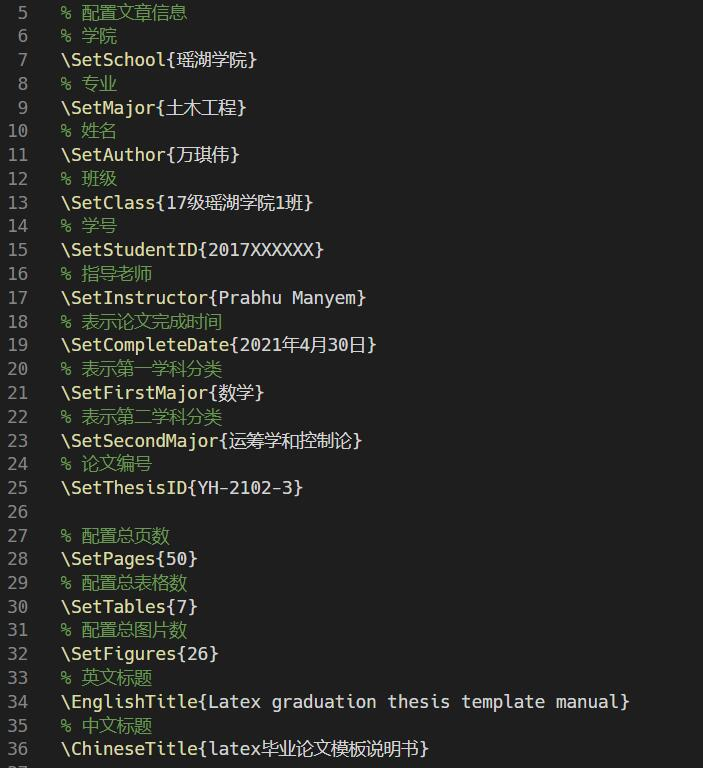
\includegraphics[width=0.65\linewidth]{information.jpg}
    \caption{待填信息}
    \label{fig.Information}
\end{figure}

\subsection{文档的基本组件}

\subsubsection{用法不变的组件}

为了减少使用难度,本模板的正文内容同一般的\LaTeX 文档一样撰写即可,包括但不限于:有序列表-enumerate,无序列表-itemize,单图-figure,表格-table和tabular,二级标题-subsection,三级标题-subsubsection,公式-align和equation等公式环境,代码块-lstlisting,算法-algorithm,超链接-href等常用命令。

\subsubsection{一级标题-Section}

本模板使用 \Code{$\backslash$Section\{一级标题\}} 来定义一级标题。

该一级标题会在标题开始前另起一页,同时在中文模式下会显示为\Code{第X章\ 一级标题},在英文模式下会显示\Code{Chapter X 一级标题}。该显示会同时同步至目录与偶数页的页眉。

\subsubsection{代码块-lstlisting}

代码块命令中已经包含了指定样式,但是由于文本的全局行距为1.5倍,而代码行距不需要那么大,因此需要在进入代码环境时前后需要输入\Code{$\backslash$linespread\{1\}}来调整当前行距和还原当前行距。如下所示:

这是1.5倍行距时的代码样式:

\begin{lstlisting}[language=C]
    # include<stdio.h>
    int main(){
        print("Hello World");
        return 0;
    }
\end{lstlisting}

这是调整行距后的代码样式:

\linespread{1}
\begin{lstlisting}[language=C]
    # include<stdio.h>
    int main(){
        print("Hello World");
        return 0;
    }
\end{lstlisting}
\linespread{1.5}

代码块的背景颜色为灰色\Code{gray},\Code{RGB=\{0.92, 0.92, 0.92\}}。

\subsubsection{行内代码-Code}

行内代码\Code{$\backslash$Code\{your code\}}命令提供一种行内代码的格式化形式,其产生一个淡灰色边框和深粉色等宽字体,用于在行间插入小片段代码或强调某个名词。

该命令存在一个比较重要的问题---不会主动换行,因此为了防止使用此命令会溢出文本边界,如上面\ref{sec.1.1.1}所示,不要使用太长的内容作为代码块插入到文档中,若必须使用大段代码,则应使用代码块环境。

\subsubsection{参考文献的插入}

本模板支持两种参考文献的插入方式,第一种是通过\Code{thebibliography}环境中插入,如下代码所示;第二种是通过\Code{bib}参考文献数据库的形式插入。

\begin{lstlisting}
    \begin{thebibliography}{99}
        ......
    \end{thebibliography}
\end{lstlisting}

如果需要指定参考文献的插入位置,在需要插入参考文献的位置处使用\Code{$\backslash$bibfile}命令,用法如下:

\begin{lstlisting}
    \bibfile{Reference.bib}
\end{lstlisting}

其中,\Code{Reference.bib}为你的参考文献数据库文件名。

\subsubsection{参考文献的引用}

本模板使用上标的形式引入参考文献,使用\Code{$\backslash$UpCite\{2019Path\}}的方式引入参考文献,该引用方式会自动生成上标,如此处\UpCite{2019Path}所示。如果不需要上标引用,则可以直接使用\Code{$\backslash$cite\{2019Path\}}命令,该引用方式不会生成上标,如此处\cite{全权2020低空无人机交通管理概览与建议}所示。

\subsubsection{插入摘要和关键词}

使用\Code{$\backslash$MakeAbstract}插入摘要和关键词,该命令会使用\Code{include}命令将文件 \Code{Abstract.tex} 和 \Code{CHAbstract.tex} 文件的内容插入到主文档中。中英文摘要的顺序会根据中英文模式进行调整:

\begin{enumerate}
    \item 中文模式:中文摘要在前,英文摘要在后
    \item 英文模式:英文摘要在前,中文摘要在后
\end{enumerate}

\subsubsection{如何插入英文摘要和关键词}

英文摘要和关键词的内容写在\Code{Abstract.tex}文件中。

英文摘要使用\Code{$\backslash$begin\{Abstract\} ... $\backslash$end\{Abstract\}}方式输入,其中摘要的行文格式与正文相同,可以直接分段和输入其他命令标识。

英文关键词使用\Code{$\backslash$begin\{KeyWords\} ... $\backslash$end\{KeyWords\}}的方式输入,建议一行输完,每个关键词使用\Code{;}分隔,相邻两个关键词之间空一个空格,就像这样:\Code{word1; word2}。当然也可以一行一个,记得每行带上一个分号同时注意空格。

\subsubsection{如何插入中文摘要和关键词}

中文摘要和关键词的内容写在\Code{CHAbstract.tex}文件中。

中文摘要使用\Code{$\backslash$begin\{CHAbstract\} ... $\backslash$end\{CHAbstract\}}方式输入,用法同英文摘要。

中文关键词使用\Code{$\backslash$begin\{CHKeyWords\} ... $\backslash$end\{CHKeyWords\}}的方式输入,用法同英文关键词。

中英文的摘要可以改变顺序,具体顺序同在文档中出现的先后顺序一样。

\subsubsection{插入目录}

插入目录使用\Code{$\backslash$MakeContent}命令,一行代码即可,将此代码直接插入到想要插入目录的位置即可。具体使用效果请看本教程的源代码。

\subsubsection{插入论文总结}

在论文总结\Code{summary.tex}文件中写好致谢内容后,在需要插入论文总结页面的地方加上如下代码:\Code{$\backslash$include\{summary\}}即可。

\subsubsection{插入致谢}

在致谢文件\Code{acknowledgement.tex}文件中写好致谢内容后,在需要插入致谢页面的地方加上如下代码:\Code{$\backslash$include\{acknowledgement\}}即可。

\subsubsection{插入本科期间发表的论文}

在本科论文文件\Code{undergraduatethesis.tex}文件中的列表环境中写好你的参考文献列表之后,在需要插入本科期间发表论文的地方加上如下代码:\Code{$\backslash$include\{undergraduatethesis\}}即可。

\subsubsection{插入附录}

在附录文件\Code{appendix.tex}文件中写好附录内容后,在需要插入附录页面的地方加上如下代码:\Code{$\backslash$include\{appendix\}}即可。

附录使用不同的标题格式,使用\Code{$\backslash$AppendixSection\{\}}命令,该命令会生成附录的一级标题,该标题不会显示在目录上,其开头以大写字母A,B,C进行编号。

使用\Code{$\backslash$AppendixSubSection\{\}}命令生成附录的二级标题,该标题不会显示在目录上,其开头以附录一级标题加上二级标题的序号组成,比如在序号为A的一级附录标题下的第二个二级附录标题,它将会显示为:\Code{A-2}。没有设置附录三级标题。

\subsubsection{以上可自由待插入内容先后顺序}

当你的论文包含以上所有部分时,必须按照如下顺序进行插入:

\begin{enumerate}
    \item 毕业设计(论文)总结,命令:\Code{$\backslash$include\{summary\}}
    \item 参考文献,命令:\Code{$\backslash$bibfile\{reference\}}
    \item 致谢,命令:\Code{$\backslash$include\{acknowledgement\}}
    \item 本科期间发表的论文,命令:\Code{$\backslash$include\{undergraduatethesis\}}
    \item 附录,命令:\Code{$\backslash$include\{appendix\}}
\end{enumerate}

\subsection{模板附带的几类封面}

\subsubsection{毕业论文扉页}

使用\Code{$\backslash$MakeCover}命令生成毕业论文扉页,本文档的第一页即为扉页示例。一般添加在文档开始之后。

\subsubsection{瑶湖学院院级封面模板}

使用\Code{$\backslash$MakeYaohuTitlePage}命令生成瑶湖学院封面,该封面独占一页,一般添加在扉页之前。该页形式如下图所示:

\begin{figure}[H]
    \begin{center}
        
\includegraphics[width=0.8\linewidth]{Yaohutitlepage.jpg}
        \caption{瑶湖学院院级封面}
    \end{center}
\end{figure}

\subsubsection{南昌工程学院校级封面模板}

使用\Code{$\backslash$MakeSubmitPage}命令生成南昌工程学院校级封面,该封面独占一页,一般添加在扉页之前。该页形式如下图所示:

\begin{figure}[H]
    \begin{center}
        
\includegraphics[width=0.8\linewidth]{submitpage.jpg}
        \caption{南昌工程学院校级封面}
    \end{center}
\end{figure}

\subsubsection{盲审模式}

本模板已经支持盲审模式。

论文盲审需要将毕业论文的个人信息等隐去,直接在本文档的开头加入\Code{$\backslash$BlindTrialMode}命令即可,该命令会将封面中的个人信息隐去。但是如果文中出现了个人信息需要手动修改,同时有的学院要求盲审不要加入致谢页面,此时需要手动删除致谢页面。

\subsection{中英文论文切换}

使用\Code{$\backslash$ChineseMode}来开启中文论文模式,不使用该命令则默认为英文论文模式。该命令一般插入在文档类型申明之后,插入位置如下面所示:

\begin{lstlisting}
\documentclass{nitthesis}
% 开启中文模式
\ChineseMode
\end{lstlisting}

中文模式与英文模式的主要区别是在前述几种封面上显示的标题不同,中文模式显示中文标题,英文模式显示英文标题。一级标题的不同,中文模式显示“第X章”,英文模式显示"Chapter X",同时这些不同的显示方式会影响页眉。目录名称、参考文献名称、致谢名称等不同,中文模式致谢显示“致谢”,英文模式致谢显示"Acknowledgement",同时会影响页眉。摘要的顺序不同,中文模式中中文摘要应该在英文摘要之前;英文模式中中文摘要应该在英文摘要之后。

\subsection{常用组件示例}

以下是一些常用的组件示例

\subsubsection{表格示例}

\begin{table}[H]
    \centering
    \caption{Notation}
    \label{table.example}
    \begin{tabular}{cp{12cm}}
        \toprule
        \centering
        \textbf{Symbol}    & \textbf{Meaning}                                                                             \\
        \midrule
        $N$                & The set of all available nodes, $n \in N$                                                    \\
        $NB_n$             & The set of all adjacent node of a node n                                                     \\
        $NA$               & The set of the nodes which has been already passed                                           \\
        $ND$               & The set of the nodes which has been determined to go through                                 \\
        $(Node_i, Node_j)$ & The ordered number pair that represents a path                                               \\
        \bottomrule
    \end{tabular}
\end{table}

\subsubsection{跨页长表格示例}

跨页长表格有一个特点:对于同一个表格,在不同的页上需要保证表头能够在每一页的分表上相同。根据此规律建立长表格生成方法,使用\Code{longtable}环境生成长表格。使用\Code{$\backslash$endhead}定义表格中每页需要出现的表头。一个简单示例如下所示:

\linespread{1}
\begin{lstlisting}
    \begin{longtable}{cp{12cm}}   % 申明长表格环境
        \caption{Notation}  % 表格标题
        \label{table.longtable}    \\
        \toprule    % 表格上部粗线
        \textbf{Symbol}    & \textbf{Meaning}                                                                             \\
        \midrule
        \endhead    % \endhead 以上的部分为在不同页中都显示的表头
        
        \bottomrule 
        \endfoot    % \endfoot 以上的部分为在不同页中都显示的表尾,这里显示的是粗横线
        $N$                & The set of all available nodes, $n \in N$                                                    \\
        $NB_n$             & The set of all adjacent node of a node n                                                     \\
        $NA$               & The set of the nodes which has been already passed                                           \\
        $ND$               & The set of the nodes which has been determined to go through                                 \\
        $(Node_i, Node_j)$ & The ordered number pair that represents a path                                               \\
        $(Node_i, Node_j)$ & The ordered number pair that represents a path                                               \\
        $(Node_i, Node_j)$ & The ordered number pair that represents a path                                               \\
        $(Node_i, Node_j)$ & The ordered number pair that represents a path                                               \\
        $(Node_i, Node_j)$ & The ordered number pair that represents a path                                               \\
        $(Node_i, Node_j)$ & The ordered number pair that represents a path                                               \\
        $(Node_i, Node_j)$ & The ordered number pair that represents a path                                               \\
        $(Node_i, Node_j)$ & The ordered number pair that represents a path                                               \\
        $(Node_i, Node_j)$ & The ordered number pair that represents a path                                               \\
        $(Node_i, Node_j)$ & The ordered number pair that represents a path                                               \\
        $(Node_i, Node_j)$ & The ordered number pair that represents a path                                               \\
        $(Node_i, Node_j)$ & The ordered number pair that represents a path                                               \\

    \end{longtable}
\end{lstlisting}
\linespread{1.5}

上文长表格的输出示意图如下表所示:

\begin{longtable}{cp{12cm}}   % 申明长表格环境
    \caption{Notation}  % 表格标题
    \label{table.longtable}    \\
    \toprule    % 表格上部粗线
    \textbf{Symbol}    & \textbf{Meaning}                                                                             \\
    \midrule
    \endhead    % \endhead以上的部分为在不同页中都显示的表头
    
    \bottomrule 
    \endfoot    % \endfoot以上的部分为在不同页中都显示的表尾,这里显示的是粗横线
    $N$                & The set of all available nodes, $n \in N$                                                    \\
    $NB_n$             & The set of all adjacent node of a node n                                                     \\
    $NA$               & The set of the nodes which has been already passed                                           \\
    $ND$               & The set of the nodes which has been determined to go through                                 \\
    $(Node_i, Node_j)$ & The ordered number pair that represents a path                                               \\
    $(Node_i, Node_j)$ & The ordered number pair that represents a path                                               \\
    $(Node_i, Node_j)$ & The ordered number pair that represents a path                                               \\
    $(Node_i, Node_j)$ & The ordered number pair that represents a path                                               \\
    $(Node_i, Node_j)$ & The ordered number pair that represents a path                                               \\
    $(Node_i, Node_j)$ & The ordered number pair that represents a path                                               \\
    $(Node_i, Node_j)$ & The ordered number pair that represents a path                                               \\
    $(Node_i, Node_j)$ & The ordered number pair that represents a path                                               \\
    $(Node_i, Node_j)$ & The ordered number pair that represents a path                                               \\
    $(Node_i, Node_j)$ & The ordered number pair that represents a path                                               \\
    $(Node_i, Node_j)$ & The ordered number pair that represents a path                                               \\
    $(Node_i, Node_j)$ & The ordered number pair that represents a path                                               \\

\end{longtable}

\subsubsection{公式示例}

\LaTeX{}有规定的公式符号语言,本模板加入了数学公式的入门教程,是英文文档。在文件夹\Code{doc}中,名字叫做\href{doc/The LaTeX Mathematics Companion-Gai.pdf}{\Code{The LaTeX Mathematics Companion-Gai.pdf}}。

\begin{align}
    \text{Minimise:} \mathop {\sum \sum }\limits_{i,j \in N} {x_{i,j}}
\end{align}

\textbf{Constraints}

\begin{align}
    {x_{i,j}} \le 1,\forall i,j \in N
\end{align}

\subsubsection{伪代码示例}

The pseudo-code representation of the algorithm is as algorithm \ref{alg.AAlgorithm}:

\begin{algorithm}
    \caption{Using A* algorithm to find out the shortest path between two nodes}
    \hspace*{0.02in} {\bf Input:}
    Read all nodes from the file, and the adjacency between the nodes\\
    \hspace*{0.02in} {\bf Output:}
    output The shortest path with the node chain.
    % \algsetup{indent=2em}
    \begin{algorithmic}[1]
        \State $Node Map$ <- information of all nodes from the map file.
        \State $Node List$ <- $Empty$ \Comment{Store a list of previous nodes and distances}
        \While {$Destination Node$ is not in $Node List$}
            \If {$Node List$ is equal to $Empty$}
                \State $Node List$ add $Starting Node$
                \State The distance from this node to the starting node is $0$
                \State Continue
            \EndIf
            \State Find the nodes which are the adjacent nodes of the nodes in $Node List$, add them into $Node List$
            \State Calculate the distance of from node in $Node List$ to the $Starting Node$
            \State Drop the node whose all adjacent nodes are in the $Node List$
        \EndWhile

        \State $Current Node$ <- $Destination Node$
        \State $Path List$ <- $Empty$
        \State $Path List$ add $Destination Node$

        \While {$Current Nodes$ == $Starting Node$}
            \State Find the shortest distance node in the adjacency nodes of $Current Node$
            \State $Path List$ add $Current Node$
        \EndWhile
        \State $Path List$ add $Starting Node$
    \end{algorithmic}
    \label{alg.AAlgorithm}
\end{algorithm}

\subsubsection{行内公式示例}

Therefore, if the starting node and the end node are too far apart, the radius of the radiation circle will increase accordingly. It can be estimated that when the straight line distance between the selected start node and the end node is $r$, the search area of A* algorithm is $A = \pi * r ^ 2$. When the radius $r$ increases by one unit, the computational complexity of the algorithm increases $\Delta A = \frac{{\partial (\pi {r^2})}}{{\partial r}} + 2$. 

\subsubsection{多子图模板示例}

对某张子图进行引用:\autoref{sub.1}

\begin{figure}[H]
    \subcaptionbox{这是第一张子图\label{sub.1}}{
        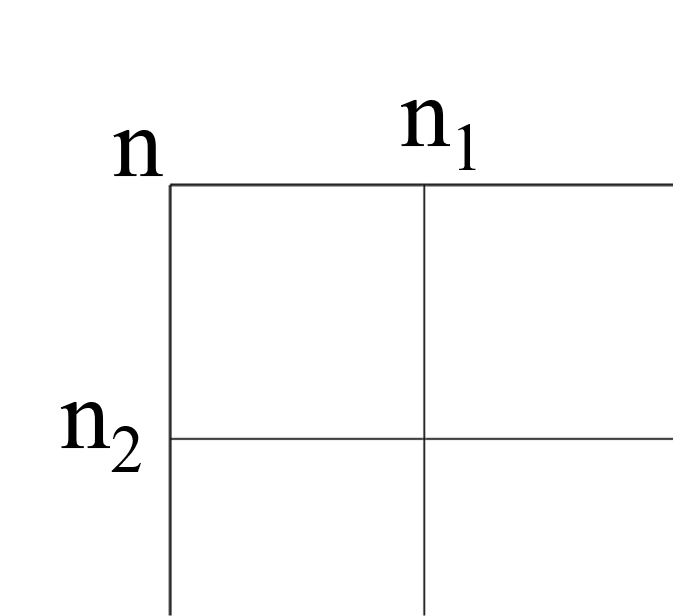
\includegraphics[width=0.3\linewidth]{adjacent node1.png}
    }
    \subcaptionbox{这是第二张子图\label{sub.2}}{
        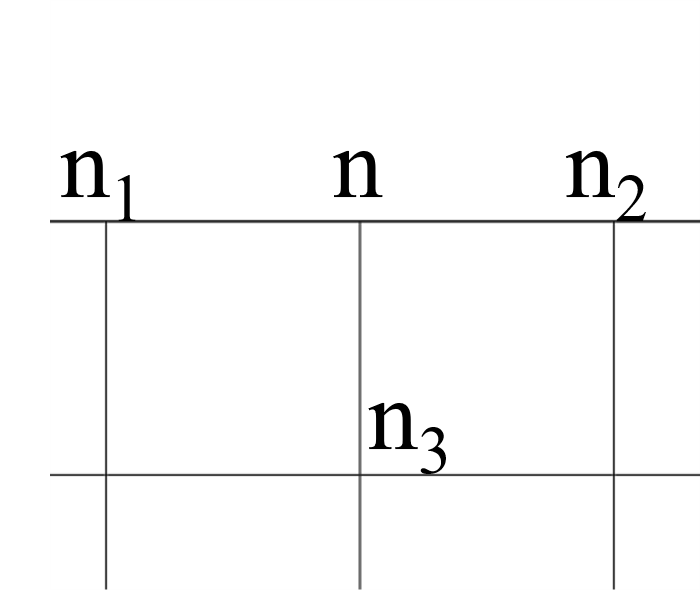
\includegraphics[width=0.3\linewidth]{adjacent node2.png}
    }
    \subcaptionbox{这是第三张子图\label{sub.3}}{
        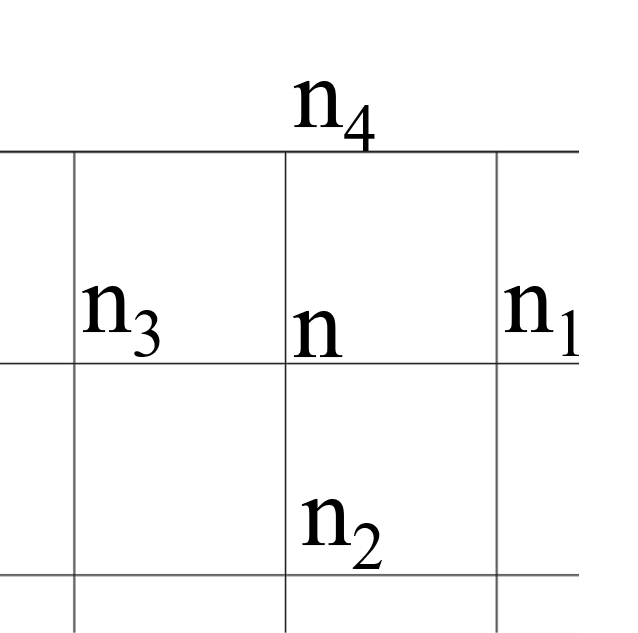
\includegraphics[width=0.3\linewidth]{adjacent node3.png}
    }
    \caption{这是三张图的总说明}
    \label{fig.ThreeFigs}
\end{figure}

\Section{模板设计依据}

本模板参考《规范》所设计,以下将对规范的每一条内容进行分析:

\begin{enumerate}
    \item \textbf{章节编号}, 满足《规范》要求
    \item \textbf{脚注}, 直接使用\Code{$\backslash$footnote\{\}}命令即可
    \item \textbf{公式},公式编号如图\ref{equ.Range}所示,满足要求
    \item \textbf{表}, 满足要求,由于latex排版的特性,如果不是超长的表,latex会将表格排在一页中
    \item \textbf{图}, 满足要求,留空正常
    \item \textbf{页眉,页脚}, 支持奇偶页不同,页脚的页码有两种,一是古罗马数字,标记摘要等页数;二是阿拉伯数字标记正文页数
\end{enumerate}

\begin{figure}[H]
    \begin{center}
        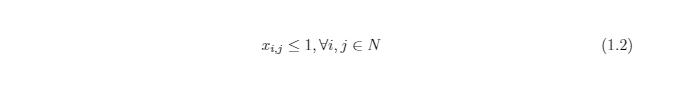
\includegraphics[width=0.96\linewidth]{equation.jpg}
        \caption{公式编号示例}
        \label{equ.Range}
    \end{center}
\end{figure}

\subsection{扉页页面格式}

\begin{enumerate}
    \item 包含三种元素:中文标题,英文标题,页面统计
    \item 中文标题在上,据页面顶端5cm,字号一号,黑体
    \item 英文标题在中文标题下距中文标题3cm,字号二号,Times New Roman
    \item 页面统计在英文标题下方12cm处,左对齐,字号小四
\end{enumerate}

\subsection{瑶湖学院院级封面格式}

\begin{enumerate}
    \item 包含四种元素,左上角全日制本科生,学位论文文字,论文信息,完成时间
    \item 全日制本科生距页顶2.5cm,五号宋体
    \item 本科学士学位论文在全日制本科生文字下方2.4cm,字号小初号,黑体,字距0.4倍字宽
    \item 论文信息在本科学士学位论文下方3.8cm处,四号宋体
    \item 完成时间在论文信息下方2.8cm处,四号黑体加粗
\end{enumerate}

\subsection{南昌工程学院校级封面格式}

\begin{enumerate}
    \item 包含六种元素,南昌工程学院字样,毕业设计字样,系院专业字样,论文题目,论文信息,完成时间
    \item 南昌工程学院字样距页顶4.5cm,小二号宋体,字距0.6倍字宽
    \item 毕业设计字样在南昌工程学院正下方(换行),一号宋体,字距0.6倍字宽
    \item 毕业论文题目在毕业设计字样下方3cm处,字号小三宋体,中文模式显示中文题目,英文模式显示英文题目
    \item 论文信息在论文题目下方3cm处,四号宋体
    \item 完成日期在论文信息下方3.2cm处,小四宋体
\end{enumerate}

\subsection{Texlive前端-TexWorks简单使用教程}

\begin{enumerate}
    \item 安装texlive套件时如果选择包含\Code{TexWorks 前端}时,会同时安装一个latex编辑器\Code{TexWorks}。安装时勾选选项如下图所示:
    \begin{figure}[H]
        \centering
        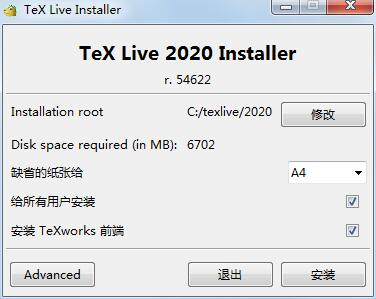
\includegraphics[width=0.7\linewidth]{forestage.jpg}
        \caption{勾选TexWorks 前端}
    \end{figure}

    \item 在安装目录下的\Code{bin/win32}文件夹中有 \Code{TexWorks} 可执行程序,双击运行,如下图所示:
    \begin{figure}[H]
        \centering
        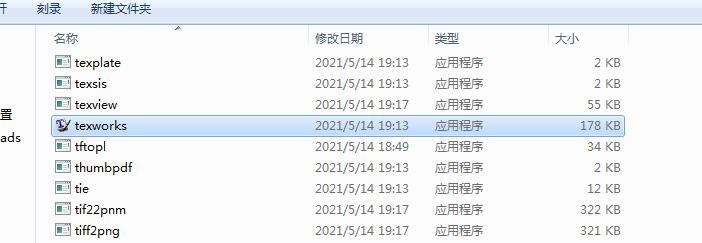
\includegraphics[width=0.9\linewidth]{dirs.jpg}
        \caption{找到TexWorks编辑器}
    \end{figure}
    
    \item 启动 \Code{TexWorks} 前端,在弹出的界面中选择打开\Code{demo}文件,如下图所示:
    \begin{figure}[H]
        \centering
        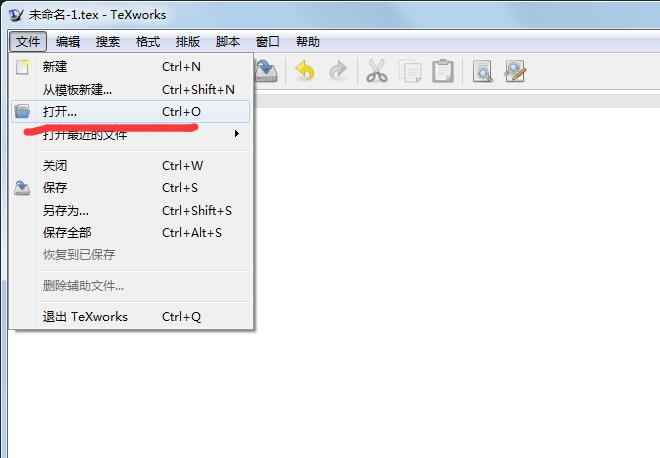
\includegraphics[width=0.6\linewidth]{openfile.jpg}
        \caption{选择打开文件}
    \end{figure}

    \item 打开\Code{demo}文档后,更换编译引擎,点击绿色三角形编译文档,编译本文档需要的引擎有两个:\Code{XeLaTeX} 和 \Code{BibTeX},如下图所示:
    \begin{figure}[H]
        \centering
        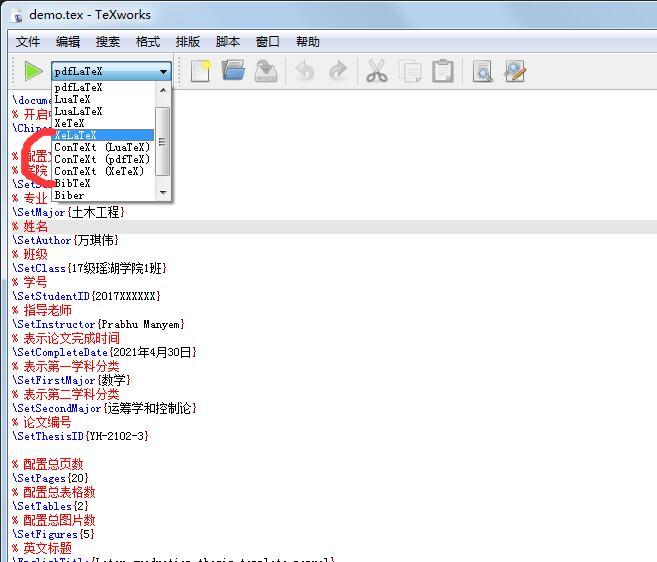
\includegraphics[width=0.7\linewidth]{chooseengine.jpg}
        \caption{更换编译引擎}
    \end{figure}

    \item 按照 \Code{XeLaTeX  ->  BibTeX  ->  XeLaTeX  ->  XeLaTeX} 分四次先后编译文档,即可生成 \Code{demo.pdf} 文件。
    
\end{enumerate}

% 论文总结
\begin{Summary}

    愉快的毕业论文模板开发就这样愉快地结束了,在这整个过程中离不开老师和其他朋友们的帮助。

    本毕业论文模板历经了不少的修修补补,最终才呈现出大家目前所看到的样子,我希望大家在使用的过程中可以向开发者多多提供意见,邮箱:\href{mailto:qi5516@qq。com}{qi5516@qq。com}

\end{Summary}
% 参考文献
\bibfile{reference}
% 致谢
\begin{Acknowledgement}

    A graduation thesis has been scattered for more than three months. 
    Since I was idle at home early last spring. 
    I have already started to do some optimization modeling problems with Mr. Prabhu. At that time, I was young and energetic, full of self-confidence in the desire for unknown territory. 
    In fact, the state at that time was that I didn't know anything and dared to do anything. 
    
    ...
    
    I would also like to thank the review experts and teachers who have taken the time to read this article.
    
\end{Acknowledgement}
% 本科期间发表的论文
\begin{UndergraduateThesis}

    \begin{enumerate}[{label=[\arabic*]}]
        \item 万琪伟,卢成林.基于HTTP1.1的WebSocket协议的新式网络聊天室设计与研究[J].通信技术,2018,51(12):3038-3042.
    \end{enumerate}

\end{UndergraduateThesis}
% 附录
\begin{Appendix}

    这里是附录示例

    \AppendixSection{Algorithm code for generating sample maps and searching for appropriate station locations}
    
    \theAppendixSubSection{Generate a map array}
    
    \begin{lstlisting}[language=C]
#include <stdio.h>
#include <stdlib.h>
        
int main()
{
    int m = 20, n = 20, d = 20, i, j, l = 20, a, b;
    int t[] = {1, 1, 0, 0, 0, 0, 0, 0, 0, 0};
    FILE *fp = fopen("example.map", "w+");
    fprintf(fp, "%d %d %d %d\n", m, n, d, l);
    for (i = 0; i < m; i++)
    {
        for (j = 0; j < n; j++)
        {
            a = rand() % 10;
            if (t[a])
                fprintf(fp, "%d", rand() % 30);
            else
                fprintf(fp, "0");
            if (j == n - 1)
                fprintf(fp, "\n");
            else
                fprintf(fp, "\t");
        }
    }
    fclose(fp);
    return 0;
}
    \end{lstlisting}

\end{Appendix}

\end{document}